\documentclass[titlepage,a4paper]{article}

\usepackage{a4wide}
\usepackage[colorlinks=true,linkcolor=black,urlcolor=blue,bookmarksopen=true]{hyperref}
\usepackage{bookmark}
\usepackage{fancyhdr}
\usepackage[spanish]{babel}
\usepackage[utf8]{inputenc}
\usepackage[T1]{fontenc}
\usepackage{graphicx}
\usepackage{float}
\usepackage{listings}
\usepackage{xcolor}

																	% VARIABLES 

\newcommand{\FirstName}{Carlos E.}
\newcommand{\LastName}{Castillo}
\newcommand{\StudentID}{108535}
\newcommand{\StudentEmail}{ccastillo@fi.uba.ar}
\newcommand{\ProjectName}{Trabajo Práctico 2 — Simulador}
% \newcommand{\ProjectName}{TDA 3 — Hash}

\pagestyle{fancy}
\fancyhf{}
\fancyhead[L]{TP - \FirstName \LastName}
\fancyhead[R]{Algoritmos y Programación II - FIUBA}
\renewcommand{\headrulewidth}{0.4pt}
\fancyfoot[C]{\thepage}
\renewcommand{\footrulewidth}{0.4pt}

\definecolor{codegreen}{rgb}{0,0.6,0}
\definecolor{codegray}{rgb}{0.5,0.5,0.5}
\definecolor{codepurple}{rgb}{0.58,0,0.82}
\definecolor{backcolour}{rgb}{0.95,0.95,0.92}

\lstdefinestyle{mystyle}{
    backgroundcolor=\color{backcolour},   
    commentstyle=\color{codegreen},
    keywordstyle=\color{magenta},
    numberstyle=\tiny\color{codegray},
    stringstyle=\color{codepurple},
    basicstyle=\ttfamily\footnotesize,
    breaklines=true,                 
    captionpos=b,                    
    keepspaces=true,                 
    numbers=left,                    
    numbersep=5pt,                  
    tabsize=4
}

\lstset{style=mystyle}

\begin{document}
\begin{titlepage}
	\hfill
\includegraphics[width=6cm]{logofiuba.jpg}
    \centering
    \vfill
    \Huge \textbf{\ProjectName}
    \vskip2cm
    \Large [7541/9515] Algoritmos y Programación II\\
    Segundo cuatrimestre de 2021 
    \vfill
    \begin{tabular}{ | l | l | }
      \hline
      Alumno: & \LastName, \FirstName \\ \hline
      Número de padrón: & \StudentID \\ \hline
      Email: & \StudentEmail \\ \hline
  	\end{tabular}
    \vfill
    \vfill
\end{titlepage}

\tableofcontents
\newpage

																 % INTRODUCCION

\section{Introducción}\label{sec:intro}

El trabajo practico presenta un hospital pokemon en el que los diferentes
entrenadores pueden atender a sus pokemones. Inicialmente se provee la
información de los entrenadores ingresantes y sus pokemones a traves de un
archivo de texto. El objetivo es implementar la funcionalidad de atencion de
los pokemones en el hospital a traves de un simulador que permita gestionar
a los pacientes internados.

Dicho simulador toma control de la informacion del hospital y permite simular
una serie de eventos a traves de diferentes comandos, que ayudan a las
enfermeras del hospital a atender a cada pokemon adivinando su nivel.

Para la construcción del simulador del el hospital de pokemones se deben
utilizar algunas de las diferentes estructuras de datos estudiadas durante
el curso de la materia, identificando cual tda resulta mas conveniente para
implementar cada funcionalidad del simulador.

                          % DETALLES DE IMPLEMENTACION

\section{Detalles de implementación}\label{sec:implementacion}

La implementación de esta estructura de datos fue escrita en el lenguaje de
programación C, siguiendo la especificación del lenguaje detallada en el
estándar C99. Los archivos principales se encuentran dentro del directorio
\textbf{src} ubicada en la raíz del repositorio. 

Además se incluye un archivo \textbf{pruebas.c} en el que se encuentran
diferentes pruebas automatizadas para detectar errores en la ejecución del
programa o en la asignación, manejo y liberación de memoria dinámica. Para esto
se utiliza \textbf{gcc} como compilador y \textbf{valgrind} como herramienta de
análisis de memoria.

El trabajo practico se encuentra dividio en dos componentes principales: la
interfaz y el simulador. La implementacion de la interfaz abarca los archivos
\textbf{main.c} y \textbf{juego.c}. Por otra parte, la implementacion del
simulador se divide en los archivos \textbf{simulador.c}, en donde se encuentra
la funcionalidad base del simulador, y los archivos auxiliares
\textbf{aux\_simulador\_atencion\_pokemon.c} y
\textbf{aux\_simulador\_dificultades.c}, que almacenan funcionalidad comun
utilizada en bastantes partes del simulador.

\subsection{Simulador}

El simulador provee tres funciones principales: \lstinline{simulador_crear},
que se encarga de la creacion e inicialización de un nuevo simulador con su
respectivo hospital, \lstinline{simulador_simular_evento}, que evalua los
diferentes comandos enviados al simulador y ejecuta el evento correspondiente
a dicho comando, y finalmente \lstinline{simulador_destruir} que se encarga de
la destruccion del simulador y liberacion de la memoria ocupada por el mismo.

La estructura propuesta para el simulador es la siguiente:

\begin{lstlisting}[language=C]
struct simulador {
	hospital_t* hospital;
	EstadisticasSimulacion estadisticas;

	heap_t* recepcion;
	lista_iterador_t* sala_espera_entrenadores;
	lista_iterador_t* sala_espera_pokemones;
	PokemonEnRecepcion* pokemon_en_tratamiento;

	abb_t* dificultades;
	DatosDificultadConId dificultad_en_uso;
	unsigned intentos_actuales;

	bool en_curso;
};
\end{lstlisting}

El primer campo \lstinline{hospital} hace referencia al hospital que se utiliza
con el simulador. Este ultimo obtiene la informacion de los registros de
ingresos de entrenadores y pokemones guardados previamente en el hospital antes
de que estos sean cargados por turnos a la simulacion. El campo
\lstinline{estadisticas} le permite al simulador llevar control sobre los
el estado actual de la simulacion, almacenando datos como el numero total de
entrenadores y pokemones, la cantidad de pokemones atendidos y en espera, entre
otras estadisticas de la simulacion en curso.

Los campos \lstinline{dificultad_en_uso}, \lstinline{intentos_actuales} y
\lstinline{en_curso} permiten al simulador mantener una referencia a ciertos
datos del estado actual de la simulacion que son de utilidad en algunos de los
eventos registrados en el simulador.

\subsection{Atención de Pokemones}

\subsubsection{Registro en Hospital}

Inicialmente los entrenadores esperan pacientemente junto con sus pokemones en
la sala de espera del hospital. Para almacenar esta informacion en el hospital
se utilizan tres estructuras de datos diferentes: dos listas enlazadas y un
árbol binario de búsqueda. Las listas enlazadas son de utilidad para guardar un
registro de los entrenadores que van ingresando al simulador en el orden de
llegada de los mismos al hospital, que es el mismo orden en el que los
entrenadores son cargados al simulador. Al utilizar una lista enlazada este
orden se respeta, ya que los elementos se almacenan en nodos dispuestos uno
tras otro de manera consecutiva, en el orden en el que van siendo insertados.
Precisamente por esta razón, en este caso la operación de inserción en la lista
enlazada solamente se hace al final de la lista para cada nuevo elemento, en vez
de hacer una inserción en posiciones específicas.

\begin{figure}[H]
\centering
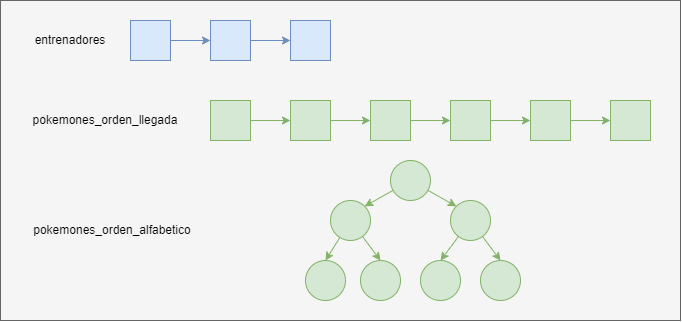
\includegraphics[width=0.9\textwidth]{img/1_hospital.png}
\caption{\label{fig:seq01}Estructura del hospital.}
\end{figure}

Además de un registro lineal de los entrenadores se necesita un registro lineal
de los pokemones, de tal manera que sea facil relacionar un rango de pokemones
con un mismo entrenador, en base a la cantidad de pokemones que registró cada
entrenador al ingresar al hospital. Para esto se utiliza la segunda lista
enlazada. Finalmente, el árbol binario de búsqueda se utiliza para facilitar
la tarea de recorrer los pokemones en orden alfabético, utilizando un árbol
binario que implemente un comparador basado en los nombres de los pokemones para
que al realizar un recorrido ''inorden'' resulte en un recorrido en orden
alfabético de todos los pokemones. Si bien esta decisión implica duplicar los
datos de los pokemones almacenados, se decidieron priorizar las optimizaciones
en cuanto a la complejidad temporal sobre la complejidad de memoria, esto
haciendo referencia al alto costo temporal que tendría ordenar una lista
enlazada de pokemones solo para recorrerlos en orden alfabético.

\subsubsection{Ingreso de Entrenadores}

Como fue mencionado anteriormente, el orden en el que ''entran'' los
entrenadores en el hospital es el mismo orden en el que estos van a ser
cargados, junto con sus pokemones, en el simulador. El simulador cuenta con un
evento llamado ''AtenderProximoEntrenador'' el cual carga la
información del siguiente entrenador no atendido cada vez que se invoca dicho
evento, es decir, de cierta forma se va avanzando sobre el listado de
entrenadores en orden de llegada, cada vez que se atiende un entrenador, se
avanza al siguiente, y luego al siguiente, así hasta haber atendido a todos los
entrenadores posibles. Como el registro de entrenadores en el hospital está
implementado utilizando una lista enlazada que respeta este mismo orden, resulta
conveniente utilizar un iterador de lista enlazada que permita replicar esta
acción de avanzar al próximo entrenador de la lista cada vez que se termine de
atender a un entrenador. Dicho iterador corresponde al campo
\lstinline{sala_espera_entrenadores} presente en el simulador.

\begin{figure}[H]
\centering
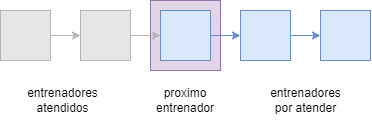
\includegraphics[width=0.65\textwidth]{img/2_iterador_entrenadores.png}
\caption{\label{fig:seq02}Registro de entrenadores con iterador de lista.}
\end{figure}

Esta funcionalidad está implementada en la función \lstinline{simulador_atender_proximo_entrenador} que toma el elemento actual del iterador
de entrenadores, es decir, el próximo entrenador a atender, y agrega todos sus
pokemones a la recepción del simulador. Para identificar cuáles son los
pokemones del hospital que pertenecen a cada entrenador, al momento de registrar
a cada entrenador se almacena como dato la cantidad de pokemones que trajo
consigo cuando ingresó al hospital. De esta forma, para un entrenador con $x$
pokemones, se pueden realizar $x$ iteraciones sobre la segunda lista enlazada
que almacena los pokemones del hospital en orden de ingreso, nuevamente
utilizando un iterador de lista enlazada, en este caso almacenado en el
campo \lstinline{sala_espera_pokemones}. 

\begin{figure}[H]
\centering
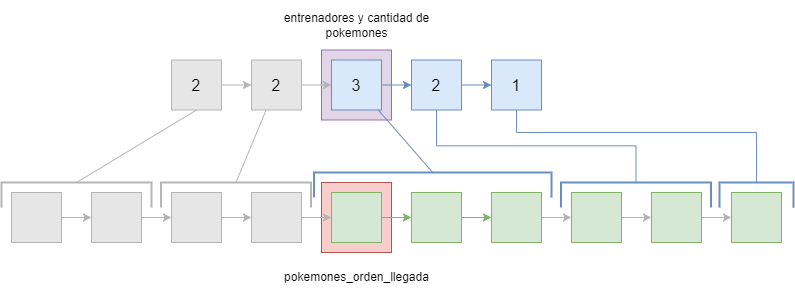
\includegraphics[width=0.9\textwidth]{img/3_pokemones_de_entrenador.png}
\caption{\label{fig:seq03}Utilización de contador e iterador de pokemones.}
\end{figure}

Al utilizar un iterador sobre la lista
enlazada de pokemones, se evitan posibles problemas que podrían ocurrir si se
usaran índices para acceder a los pokemones por entrenador en una sola lista, ya
que cada vez que se avanza el iterador, el elemento actual del mismo se deja en
la posición que corresponde al inicio del rango de pokemones del siguiente
entrenador, asegurando así que los pokemones de un entrenador ''interfieran''
con los pokemones de otro por un error de indexado. Además, esta implementación
de iterador + contador de pokemones (por entrenador) permite reducir la
complejidad del código y la complejidad temporal que se tendría de utilizarse 
otra estructura de datos como una doble lista enlazada (una lista enlazada de
pokemones por cada entrenador en una lista enlazada de entrenadores). Para esto
último se utilizan las funciones auxiliares
\lstinline{simulador_atender_pokemon_de_menor_nivel} y
\lstinline{aux_agregar_pokemones_de_entrenador_a_recepcion} que ayudan a
modularizar	un poco el proceso de guardado de los pokemones de cada entrenador.

\subsubsection{Recepción de Pokemones}

El simulador está diseñado para que cada vez que se atienda a un nuevo pokemon,
siempre se elija aquel pokemon que tenga el menor nivel posible entre todos los
ya cargados al simulador. Esto implica que cada vez que se atiendan nuevos
entrenadores y estos pasen sus pokemones al simulador, dichos pokemones se 
deben almacenar en una estructura de datos que sea capaz de mantener el orden
tras cada inserción, de tal forma que se garantice que en cuanto haya espacio
disponible en el consultorio para atender a un pokemon, sea efectivamente el 
pokemon de menor nivel el que pase a ser atendido, sin verse afectado por otros
factores que podría afectar el orden en ciertas estructuras de datos como el
orden de llegada del pokemon.

Una vez establecida la necesidad de cumplir con este criterio, se hace evidente
que la estructura de datos que encaja mejor con la funcionalidad requerida es 
el heap binario minimal. Esta estructura de datos es un árbol binario que
mantiene en su raíz al menor de todos los elementos basados en el criterio de
comparación deseado, en este caso el nivel del pokemon. De esta forma, cada vez
que se desea seleccionar el próximo pokemon a ser atendido, solo se extrae la
raíz del heap, que en el caso del simulador corresponde al campo
\lstinline{recepcion}, y directamente se asegura que dicha elemento extraído
es el pokemon de menor nivel entre los pokemones disponibles en toda la
recepción.

\begin{figure}[H]
\centering
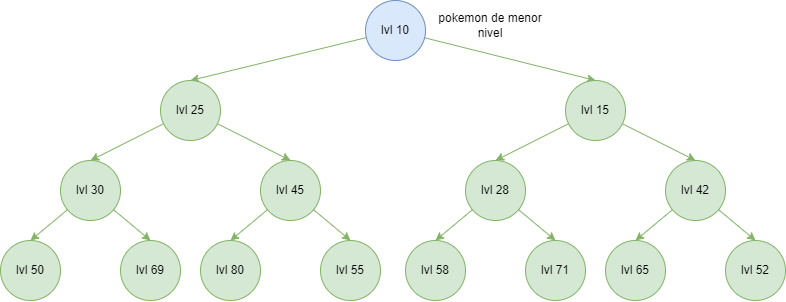
\includegraphics[width=0.9\textwidth]{img/4_heap_pokemones.png}
\caption{\label{fig:seq04}Recepción de pokemones con heap binario.}
\end{figure}

Para atender a un pokemon enlistado cuando hay espacio disponible en el
consultorio, se utiliza la función auxiliar
\lstinline{simulador_atender_pokemon_de_menor_nivel}, que tal y como su nombre
indica, una vez que se tiene espacio disponible para avanzar al pokemon de menor
nivel para que este sea atendido, se encarga de destruir el pokemon que estaba
actualmente en el consultorio (si es que había uno), extrae la raíz del heap
que almacena todos los pokemones disponibles, y posiciona al pokemon de menor
nivel como nuevo pokemon en tratamiento. En el caso del simulador, este pokemon
es almacenado en el campo \lstinline{pokemon_en_tratamiento}.

\subsection{Manejo de Dificultades}

El objetivo del simulador es permitir que el usuario adivine el nivel de un
pokemon cuando este está siendo atendido. Esto es posible a través del evento
''AdivinarNivelPokemonEnTratamiento''. Este evento utiliza las funciones
específicas de la dificultad que esta activa en el momento en el simulador para
determinar si el intento de adivinar el nivel del pokemon hecho por el usuario
es correcto o incorrecto. Para esto es necesario tener una forma de identificar
cuál es la dificultad que se encuentra activa en el momento de realizar el
intento y cuales son las funciones de esa dificultad para calcular los puntajes, 
generar pistas y verificar los resultados de cada intento.

El simulador cuenta con un registro de las diferentes dificultades agregadas
al mismo, teniendo siempre como mínimo tres dificultades: ''Facil'', ''Media'' y 
''Dificil''. Para almacenar estas dificultades en el campo
\lstinline{dificultades} del simulador, se hace uso de un árbol binario de
búsqueda, principalmente por la eficiencia de esta estructura de datos para
buscar cierto elemento en base al criterio de ordenamiento, en este caso, buscar
dificultades en base al ID de las mismas. Sin embargo si bien sobre el papel
esta estructura presenta esta ventaja, en la práctica no resulta ni más ni
menos eficiente para la búsqueda que lo que hubiera resultado si se utilizara
una lista enlazada, dado a que a como están construidas las funciones que ayudan
a la creacion de una nueva dificultad, \lstinline{simulador_agregar_dificultad}
junto con otros auxiliares como \lstinline{crear_dificultad}, el ID de cada
nueva dificultad agregada se auto-genera a partir de la cantidad de dificultades
ya existentes, de tal manera que el ID de la nueva dificultad siempre va a ser
mayor que los IDs existentes y por lo tanto el árbol binario de búsqueda se 
termina degenerando en una lista enlazada. Sin embargo se decidió conservar la
implementación de árbol binario en caso de que se desee cambiar la
auto-generación de los IDs en un futuro y también porque provee directamente
la primitiva \lstinline{abb_buscar}, para buscar una dificultad por ID cuando se 
desea cambiar la dificultad del simulador.

\begin{figure}[H]
\centering
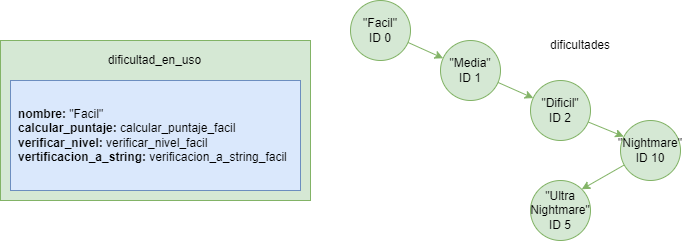
\includegraphics[width=0.9\textwidth]{img/5_dificultades.png}
\caption{\label{fig:seq05}Dificultades del simulador.}
\end{figure}

Una vez se cambia la dificultad del simulador, al momento de intentar adivinar
el nivel del pokemon en tratamiento nuevamente, el evento tomará en
consideración las funciones de verificación del intento correspondientes a la
dificultad con la dificultad activa, almacenada en el simulador dentro del campo
\lstinline{dificultad_en_uso}. El simulador también lleva control sobre la
cantidad de intentos requeridos hasta adivinar el nivel de un pokemon cada vez
que se inicia dicho evento. Este datos es requerido por algunas dificultades
para calcular el puntaje final.

\subsection{Interfaz}

La parte de la interfaz (tambien llamado juego) hace las veces de cliente para
el simulador. Provee al usuario una forma de ingresar comandos y controlar el
simulador, asi como tambien intentar adivinar el pokemon en tratamiento, sin
embargo el simulador sigue siendo independiente de la interfaz y puede funcionar
perfectamente sin la misma.

El iniciarse el juego primero se cargan los datos del hospital correspondiente
al archivo de registros de ingresos dado y luego se inicializa una instancia del
simulador con estos datos, todo esto utilizando la funcion
\lstinline{juego_inicializar}. También se agregan dos dificultades adicionales: 
''Nightmare'' y ''Ultranightmare'' para hacer mas entretenido el intentar
adivinar el nivel del pokemon que esté en tratamiento. El funcionamiento basico
de este juego consiste en una linea de comandos que luego de ejecutar el comando
anterior o el primer comando sigue pidiendo input del usuario para ejecutar otro
comando de entre las opciones disponibles.

La mayoría de los comandos presentados corresponden a un único evento del
simulador, sin embargo algunos simulador múltiples eventos para mejorar la
experiencia del usuario que utiliza el juego en comparación con cómo sería
llamar a cada uno de los eventos del simulador sin la interfaz gráfica. Por
ejemplo, el comando ''Mostrar Dificultades Disponibles'' realmente manda invoca
el evento ''ObtenerInformacionDificultad'' múltiples veces para mostrar la
información de todas las dificultades requiriendo que el usuario ingrese solo
un comando, en vez de un comando para ver la información de cada una de las 
dificultades.

Finalmente cabe destacar que para mejorar la consistencia de la interfaz y para
que el juego se vea mas llamativo, también existen algunas funciones auxiliares
como \lstinline{juego_titulo} y \lstinline{juego_prompt_exito}, que unifican la 
forma en la que se muestran los titulos a lo largo del juego.

\end{document}

